% ===========================================================
% venn_patrones_dinamicos.tex
% Diagrama de Venn ajustado para pagina tamano carta
% ===========================================================
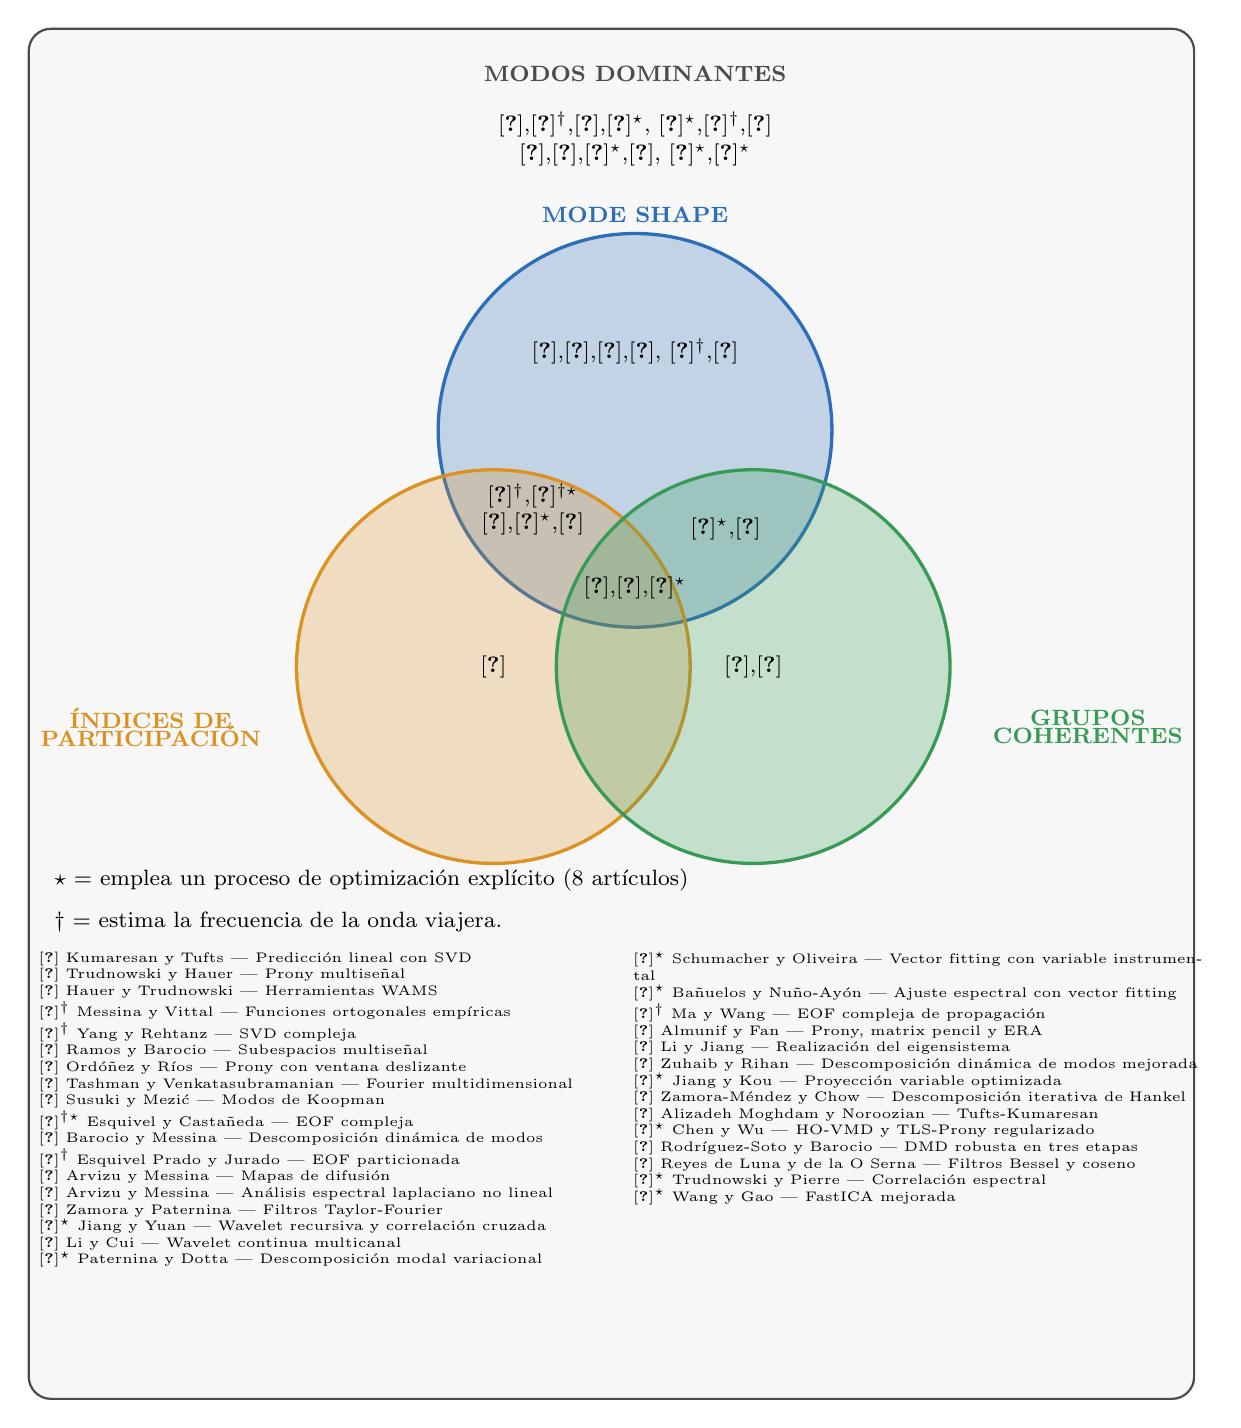
\begin{tikzpicture}[
    scale=1, transform shape, % <--- ESCALA GLOBAL PARA ENTRAR EN CARTA
    conjunto/.style={draw, very thick, fill opacity=0.26, text opacity=1},
    etiqueta/.style={font=\footnotesize\bfseries},
    art/.style={font=\footnotesize, inner sep=1pt, align=center},
    titulo/.style={font=\footnotesize\bfseries}
]

\definecolor{cFM}{RGB}{ 45,110,185}   % Formas Modales
\definecolor{cIP}{RGB}{220,145, 35}   % Indices de Participacion
\definecolor{cGC}{RGB}{ 55,155, 85}   % Grupos Coherentes

% ---------- UNIVERSO MARCO ----------
\draw[draw=black!70, thick, rounded corners=8pt, fill=black!3]
      (-11.5,-7.8) rectangle (3.3,9.6);


% ---------- CIRCULOS (CENTRO_X, CENTRO_Y) circle (RADIO) ----------
\draw[conjunto, draw=cFM, fill=cFM] ( -3.8, 4.5) circle (2.5); % Formas Modales
\draw[conjunto, draw=cIP, fill=cIP] (-5.6,1.5) circle (2.5); % Indices Participacion
\draw[conjunto, draw=cGC, fill=cGC] ( -2.3,1.5) circle (2.5); % Grupos Coherentes

% ---------- ETIQUETAS PRINCIPALES DE CONJUNTO ----------
\node[etiqueta, text=black!70, align=center] at ( -3.8, 8.90)
     {MODOS DOMINANTES\\[-2pt]};
\node[etiqueta, text=cFM, align=center] at ( -3.8, 7.1)
     {MODE SHAPE\\[-2pt]};
\node[etiqueta, text=cIP, align=center] at (-9.95,0.60)
     {\'INDICES DE\\[-3pt]PARTICIPACI\'ON\\[-2pt]};
\node[etiqueta, text=cGC, align=center] at ( 1.95,0.60)
     {GRUPOS\\[-3pt]COHERENTES\\[-2pt]};

% ---------- TEXTOS INTERIORES: SOLO MODOS DOMINANTES ----------
\node[font=\footnotesize, align=center] at (-3.8, 8.20)
  {\cite{Tufts1982},\cite{Messina2007}$^{\dagger}$,\cite{Ordonez2013},\cite{Paternina2019}$^{\star}$,
  \cite{Schumacher2019}$^{\star}$,\cite{Ma2019}$^{\dagger}$,\cite{Almunif2020}\\[1pt]
      \cite{Zamora2023},\cite{Moghdam2024},\cite{Chen2024}$^{\star}$,\cite{Rodriguez2024},
      \cite{ReyesDeLuna2025}$^{\star}$,\cite{Wang2025}$^{\star}$};

      
% ---------- TEXTOS INTERIORES: SOLO FORMAS MODALES ----------
\node[art] at (-3.8,5.50)
{\cite{Trudnowski1999},\cite{Hauer2007},\cite{Tashman2014},\cite{Susuki2014},
\cite{Esquivel2015}$^{\dagger}$,\cite{Trudnowski2025}};


% ---------- TEXTOS INTERIORES: SOLO INDICES DE PARTICIPACION ----------
\node[art] at (-5.6,1.5) 
 {\cite{Ramos2013}};

% ---------- TEXTOS INTERIORES: SOLO GRUPOS COHERENTES ----------
\node[art] at (-2.3,1.5)
{\cite{Arvizu2016},\cite{ArvizuNLSA2016}};

% ---------- INTERSECCION: FM y IP ----------
\node[art] at (-5.1,3.5)
     {\cite{Yang2012}$^{\dagger}$,\cite{EsquivelCastaneda2014}$^{\dagger\star}$\\
     \cite{Zamora2017},\cite{Banuelos2019}$^{\star}$,\cite{Zuhaib2021}
     };


% ---------- INTERSECCION: FM y GC ----------
\node[art] at (-2.65,3.25)
     {\cite{Jiang2017}$^{\star}$,\cite{Li2018}};

% ---------- INTERSECCION CENTRAL: LOS TRES CONJUNTOS ----------
\node[art] at (-3.8,2.5)
     {\cite{Barocio2015},\cite{li2020era},\cite{jiang2021}$^{\star}$};



% ---------- NOTA A PIE ----------

\node[font=\footnotesize, align=left, anchor=north west] at (-11.30,-0.95)
     { $\star$ = emplea un proceso de optimizaci\'on expl\'icito (8 art\'iculos)};


\node[font=\footnotesize, align=left, anchor=north west] at (-11.30,-1.5)
     {$\dagger$ = estima la frecuencia de la onda viajera.};

     \node[font=\tiny, align=left, anchor=north west, text width=7.25cm] at (-11.50,-2)
     {\cite{Tufts1982} Kumaresan y Tufts --- Predicci\'on lineal con SVD\\
      \cite{Trudnowski1999} Trudnowski y Hauer --- Prony multise\~nal\\
      \cite{Hauer2007} Hauer y Trudnowski --- Herramientas WAMS\\
      \cite{Messina2007}$^{\dagger}$ Messina y Vittal --- Funciones ortogonales emp\'iricas\\
      \cite{Yang2012}$^{\dagger}$ Yang y Rehtanz --- SVD compleja\\
      \cite{Ramos2013} Ramos y Barocio --- Subespacios multise\~nal\\
      \cite{Ordonez2013} Ord\'o\~nez y R\'ios --- Prony con ventana deslizante\\
      \cite{Tashman2014} Tashman y Venkatasubramanian --- Fourier multidimensional\\
      \cite{Susuki2014} Susuki y Mezi\'c --- Modos de Koopman\\
      \cite{EsquivelCastaneda2014}$^{\dagger\star}$ Esquivel y Casta\~neda --- EOF compleja\\
      \cite{Barocio2015} Barocio y Messina --- Descomposici\'on din\'amica de modos\\
      \cite{Esquivel2015}$^{\dagger}$ Esquivel Prado y Jurado --- EOF particionada\\
      \cite{Arvizu2016} Arvizu y Messina --- Mapas de difusi\'on\\
      \cite{ArvizuNLSA2016} Arvizu y Messina --- An\'alisis espectral laplaciano no lineal\\
      \cite{Zamora2017} Zamora y Paternina --- Filtros Taylor-Fourier\\
      \cite{Jiang2017}$^{\star}$ Jiang y Yuan --- Wavelet recursiva y correlaci\'on cruzada\\
      \cite{Li2018} Li y Cui --- Wavelet continua multicanal\\
      \cite{Paternina2019}$^{\star}$ Paternina y Dotta --- Descomposici\'on modal variacional};

\node[font=\tiny, align=left, anchor=north west, text width=7.25cm] at (-3.95,-2)
     {\cite{Schumacher2019}$^{\star}$ Schumacher y Oliveira --- Vector fitting con variable instrumental\\
      \cite{Banuelos2019}$^{\star}$ Ba\~nuelos y Nu\~no-Ay\'on --- Ajuste espectral con vector fitting\\
      \cite{Ma2019}$^{\dagger}$ Ma y Wang --- EOF compleja de propagaci\'on\\
      \cite{Almunif2020} Almunif y Fan --- Prony, matrix pencil y ERA\\
      \cite{li2020era} Li y Jiang --- Realizaci\'on del eigensistema\\
      \cite{Zuhaib2021} Zuhaib y Rihan --- Descomposici\'on din\'amica de modos mejorada\\
      \cite{jiang2021}$^{\star}$ Jiang y Kou --- Proyecci\'on variable optimizada\\
      \cite{Zamora2023} Zamora-M\'endez y Chow --- Descomposici\'on iterativa de Hankel\\
      \cite{Moghdam2024} Alizadeh Moghdam y Noroozian --- Tufts-Kumaresan\\
      \cite{Chen2024}$^{\star}$ Chen y Wu --- HO-VMD y TLS-Prony regularizado\\
      \cite{Rodriguez2024} Rodr\'iguez-Soto y Barocio --- DMD robusta en tres etapas\\
      \cite{ReyesDeLuna2025} Reyes de Luna y de la O Serna --- Filtros Bessel y coseno\\
      \cite{Trudnowski2025}$^{\star}$ Trudnowski y Pierre --- Correlaci\'on espectral\\
      \cite{Wang2025}$^{\star}$ Wang y Gao --- FastICA mejorada};



\end{tikzpicture}